\section{Robustness Checks}
\label{sec:robust}

\subsection{Nested model comparison}
Table~\ref{tab:nested} compares three nested versions of the structural model \eqref{eq:logit} for each criterion:
S1 with the system only, S2 adding the requested length and S3 adding the meter. Fig.~\ref{fig:nested} plots their fit.
Length adds by far the most to both models, and the meter adds a smaller but significant amount; S3 has the lowest AIC
under both criteria. The system effect alone explains about twice as much under the extended criterion as under the
base criterion, which is H1 seen from another angle: the base criterion hides most of the difference between the human
and generated poems.

\begin{table}[t]
\centering
\caption{Nested structural models (likelihood-ratio tests against the previous step). Lowest AIC per criterion in bold.}
\label{tab:nested}
\scriptsize
\setlength{\tabcolsep}{2.5pt}
\begin{tabular}{@{}l l r r r r r@{}}
\toprule
Criterion & Model & $k$ & $R^2_{\mathrm{McF}}$ & AIC & LR ($df$) & $p$ \\
\midrule
\rowsinput{generated/tab_nested.tex}
\bottomrule
\end{tabular}
\end{table}

\begin{figure}[t]
\centering
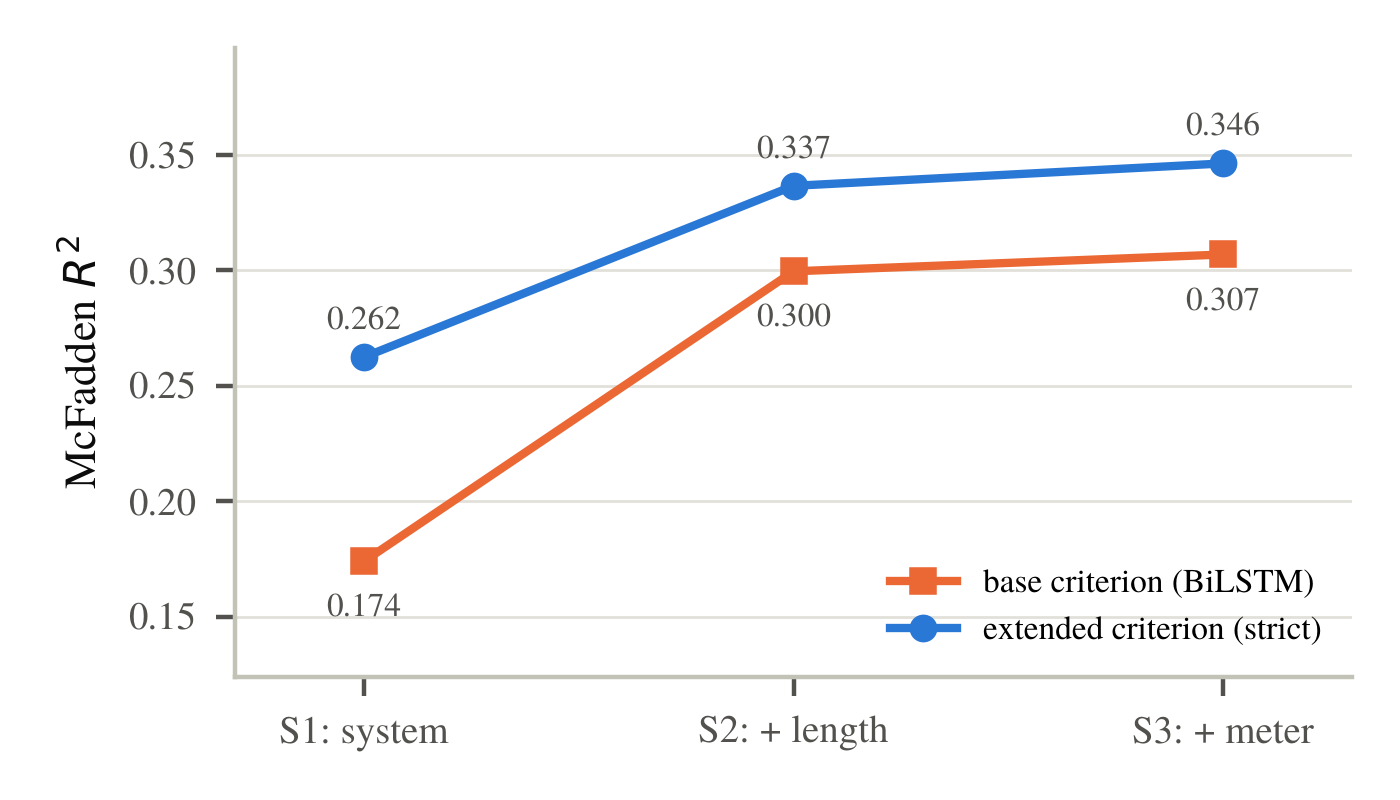
\includegraphics[width=\columnwidth]{fig_nested.png}
\caption{Fit of the nested structural models (McFadden $R^2$) for the base and the extended criterion.}
\label{fig:nested}
\end{figure}

\subsection{Alternative specifications of validity}
The extended criterion has several parts and one tuned setting, the margin $\delta$. Table~\ref{tab:variants} and
Fig.~\ref{fig:robust} recompute strict validity with one part removed or changed at a time. The gap between the human
poems and E0 survives every variant. Removing the rhyme check raises E0 the most (to \val{vEzeroNoRhyme}\%), which
confirms that rhyme is its largest weakness. Removing the length check changes little, because most length errors come
together with meter or rhyme errors. Accepting any form of the requested meter changes almost nothing. The margin
matters for human poems, whose rejections are mostly of the margin kind (Section~\ref{sec:m1}), and much less for E0,
whose failures are mostly hemistichs with no reading in the meter: without any margin, E0 rises only to
\val{vEzeroNoMargin}\% while the human poems rise to \val{vRefNoMargin}\%. So the low validity of the generated poems is
not an artefact of the margin. Binding mode is stricter for both. Finally, the base criterion passes
\val{vEzeroBaseBilstm}\% of E0 poems, eight times the strict rate.

\begin{table}[t]
\centering
\caption{Strict validity (\%) under alternative specifications. Each row changes one part of the extended criterion.}
\label{tab:variants}
\footnotesize
\setlength{\tabcolsep}{3pt}
\begin{tabular}{@{}l r r r r r r@{}}
\toprule
Specification & Human & E0 & E1 & E3 & C-wm & C-mr \\
\midrule
Full (margin 1.5) & \val{vRefFull} & \val{vEzeroFull} & \val{vEoneFull} & \val{vEthreeFull} & \val{vCwmFull} & \val{vCmrFull} \\
-- rhyme check & \val{vRefNoRhyme} & \val{vEzeroNoRhyme} & \val{vEoneNoRhyme} & \val{vEthreeNoRhyme} & \val{vCwmNoRhyme} & \val{vCmrNoRhyme} \\
-- length check & \val{vRefNoLength} & \val{vEzeroNoLength} & \val{vEoneNoLength} & \val{vEthreeNoLength} & \val{vCwmNoLength} & \val{vCmrNoLength} \\
any form of the meter & \val{vRefAnyForm} & \val{vEzeroAnyForm} & \val{vEoneAnyForm} & \val{vEthreeAnyForm} & \val{vCwmAnyForm} & \val{vCmrAnyForm} \\
margin 1.0 & \val{vRefMarginOne} & \val{vEzeroMarginOne} & \val{vEoneMarginOne} & \val{vEthreeMarginOne} & \val{vCwmMarginOne} & \val{vCmrMarginOne} \\
margin 3.0 & \val{vRefMarginThree} & \val{vEzeroMarginThree} & \val{vEoneMarginThree} & \val{vEthreeMarginThree} & \val{vCwmMarginThree} & \val{vCmrMarginThree} \\
no margin & \val{vRefNoMargin} & \val{vEzeroNoMargin} & \val{vEoneNoMargin} & \val{vEthreeNoMargin} & \val{vCwmNoMargin} & \val{vCmrNoMargin} \\
binding mode & \val{vRefBinding} & \val{vEzeroBinding} & \val{vEoneBinding} & \val{vEthreeBinding} & -- & -- \\
\midrule
base criterion (BiLSTM) & \val{vRefBaseBilstm} & \val{vEzeroBaseBilstm} & \val{vEoneBaseBilstm} & \val{vEthreeBaseBilstm} & -- & -- \\
\bottomrule
\end{tabular}
\end{table}

\begin{figure*}[t]
\centering
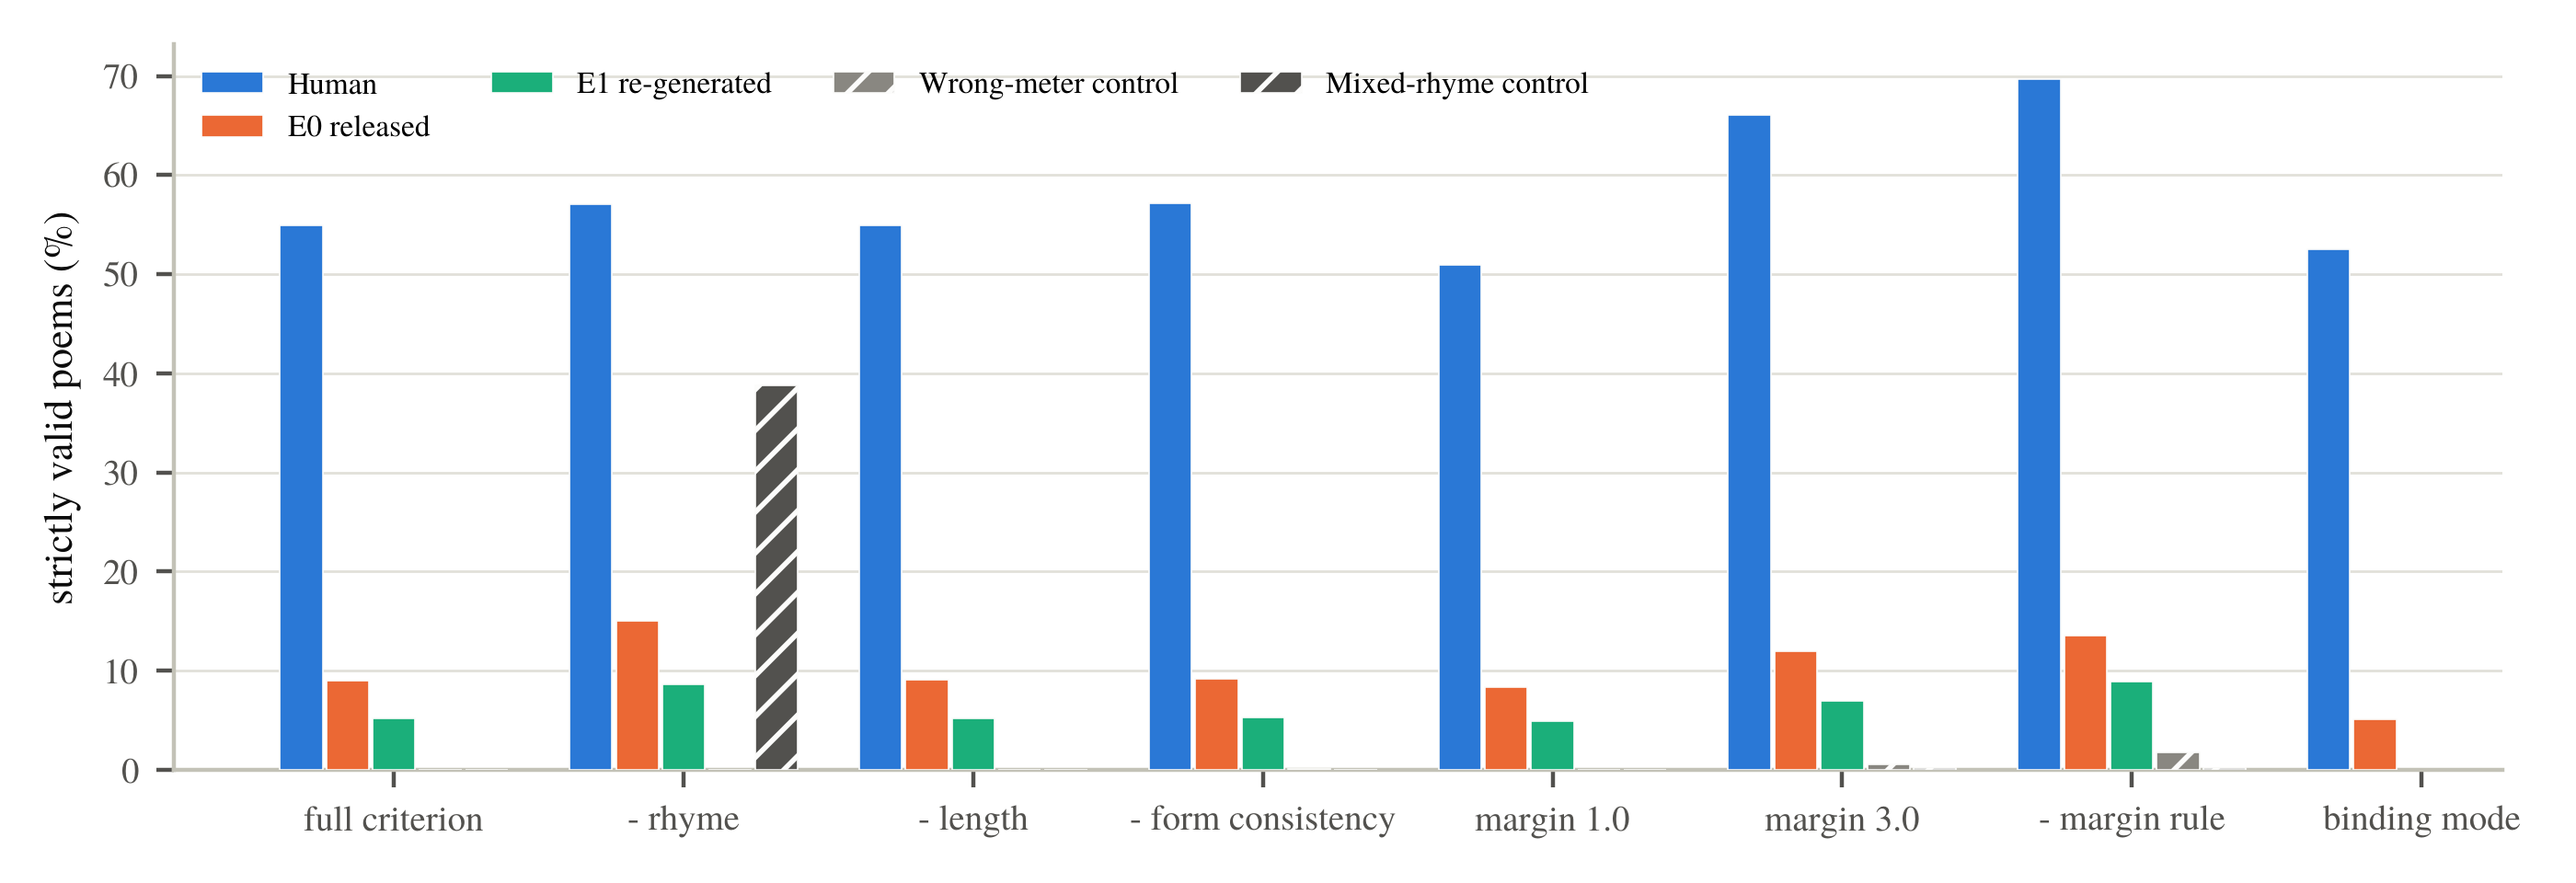
\includegraphics[width=0.8\textwidth]{fig_robustness.png}
\caption{Strict validity under the alternative specifications of Table~\ref{tab:variants}. Hatched bars are the control
samples, which stay near zero under every specification that keeps the part they break.}
\label{fig:robust}
\end{figure*}

\subsection{Subsample checks}
\textbf{Independent generations.} The findings on the released poems were repeated on our own poems, E1 (released
adapter) and E3 (re-trained). Both have a large gap between the BiLSTM and the verifier, a strict-validity rate far
below the human poems, and the same decline with length (Tables~\ref{tab:m3} and~\ref{tab:variants}).
\textbf{Short poems.} Restricted to the 1,668 prompts of 1--3 bayts, where length errors are rare, E0 is still strictly
valid for only \val{mEzeroLenA}\% against \val{mRefLenA}\% of human poems, so the gap is not produced by long poems
alone.

\subsection{Common method bias and multiple testing}
In survey research, common method bias arises when the same instrument measures both sides of a
relation~\cite{podsakoff2003cmb}. The analogue here is that the verifier both selects poems (M4, M5) and scores them.
We address it in three ways: (i) the measurement results (H1--H3) involve no selection at all; (ii) every improvement
is also scored by instruments that did not select the poems, namely the BiLSTM, the binding mode and the LLM judge
(H5); and (iii) the human study is blinded. For multiple testing, the hypotheses are grouped into families (measurement,
M4, M5, M6) and Holm's correction~\cite{holm1979simple} is applied within each family. The measurement results have
$p<0.001$ and are unaffected by the correction.
